\documentclass[xcolor ={table,usenames,dvipsnames}]{beamer}
\usepackage[italian]{babel}
\usepackage{color}
\usepackage{txfonts}
\PassOptionsToPackage{dvipsnames}{xcolor}
\title{Multivariate Analysis and Statistical Learning \\PC Algorithm's implementation}
\author{Authors: Alex Foglia, Tommaso Puccetti}
\institute{Universit\`a  degli Studi di Firenze}
\date{21/12/2018}
%\usepackage{sansmathaccent}
\usetheme{Berlin} 
\useinnertheme{rounded}
\useoutertheme{miniframes} 
\setbeamercovered{dynamic}
\theoremstyle{definition}
\newtheorem{definizione}{Definizione}
\usepackage{tikz}
\usetikzlibrary{arrows}
\usepackage{subfigure}
\begin{document}
	
	\begin{frame}
		\maketitle
	\end{frame}

	\begin{frame}
		\frametitle{Theoretical references (1)}
		\begin{itemize}
			\item Bayesian Networks can be rappresented as a \textbf{directed acyclic graph (DAG)};
			\item "acyclic" means that there are no paths starting from a node $v$ that ends with $v$ itself, $\forall v \in G$.
			
		\end{itemize}
	\end{frame}

	\begin{frame}
		\frametitle{Theoretical references (2)}
		Let $G = (V,E)$ be a DAG relative to a finite set  $X = \{X_{v}, v \in V\}$ of casual variables, then:
		$$
		\forall\; u,v \in V \;non\;adjacent\;|\; v \in nd(u) \Rightarrow 
		$$
		$$\Rightarrow u \Perp v \;|\; nd(u) - v $$
	Where $nd(u)$ is the set of \textbf{non-descendant} nodes of u, that are all those nodes $u'$ for which there is no path from $u$ to $u'$. \\
	\end{frame}

	\begin{frame}
		\frametitle{Theoretical references (3)}
		\begin{figure}
			\centering
			\subfigure[$2 \Perp 3\;|\; 1$]
			{\begin{tikzpicture}[->,>=stealth',shorten >=1pt,auto,node distance=2cm,
				thick,main node/.style={circle,draw,font=\sffamily\Large\bfseries}]
				
				\node[main node] (1) {1};
				\node[main node] (2) [below left of=1] {2};
				\node[main node] (3) [below right of=1] {3};
				
				\path[every node/.style={font=\sffamily\small}]
				
				(1) edge [right] node[left] {} (2)
				edge [right] node[left] {} (3);
				
				\end{tikzpicture}}
			\hspace{5mm}
			\subfigure[$2 \Perp 3\;|\; 1$]
			{\begin{tikzpicture}[->,>=stealth',shorten >=1pt,auto,node distance=2cm,
				thick,main node/.style={circle,draw,font=\sffamily\Large\bfseries}]
				
				\node[main node] (1) {1};
				\node[main node] (2) [below left of=1] {2};
				\node[main node] (3) [below right of=1] {3};
				
				\path[every node/.style={font=\sffamily\small}]
				
				(1) edge [right] node[left] {} (2)
				(3)edge [right] node[right] {} (1);
				
				\end{tikzpicture}}
			\hspace{5mm}
			\subfigure[$2 \not\Perp 3\;|\; 1  $  ]{\begin{tikzpicture}[->,>=stealth',shorten >=1pt,auto,node distance=2cm,
				thick,main node/.style={circle,draw,font=\sffamily\Large\bfseries}]
				
				\node[main node] (1) {1};
				\node[main node] (2) [below left of=1] {2};
				\node[main node] (3) [below right of=1] {3};
				
				\path[every node/.style={font=\sffamily\small}]
				
				(2) edge [right] node[left] {} (1)
				(3) edge [right] node[left] {} (1);
				
				\end{tikzpicture}}
		\end{figure}
		
		\begin{figure}
			
		\end{figure}
	\end{frame}


	\begin{frame}
		\frametitle{PC-Algorithm}
		Given a set of variables with a joint Gaussian probability distribution, it is possible to learn the DAG closer to the sample through the use of  \textbf{PC-Algorithm}. \\
		It is composed of two sub-functions that solve two different problems:
		\begin{enumerate}
			\item The construction of the \textbf{skeleton} from the moral graph;
			\item The construction of the DAG from a given skeleton.
		\end{enumerate}
	\end{frame}


	\begin{frame}
		\frametitle{Step 1: read the dataset}
		\begin{itemize}
			\item Import \textbf{pandas} library;
			\item call \textbf{pandas.read$\_$csv()} function to read dataset;
			\item define \textbf{alpha};
			\item call \textbf{get\_skeleton} on dataset and alpha as arguments.
		\end{itemize}
		\begin{figure}[h!]
			\centering
			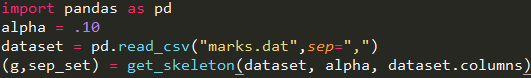
\includegraphics[scale=0.82]{img/dataset.PNG}
		\end{figure}
		
	\end{frame}
	\begin{frame}
\frametitle{Step 2: initialization}
\begin{itemize}
	\item Read names of the dataset variables accessing \textbf{dataset.columns} field;
	\item retrieve the correlation matrix of the given dataset with \textbf{dataset.corr().values};
	\item initialize \textbf{N,n} as the number of sampling and the number of variables;
	\item initialize \textbf{G} as the complete graph of dimension n;
	\item initalize the \textbf{separation\_set} as a list of list;
	\item initialize \textbf{l = 0}, \textbf{stop = false}.
\end{itemize}
	\begin{figure}[h!]
		\centering
		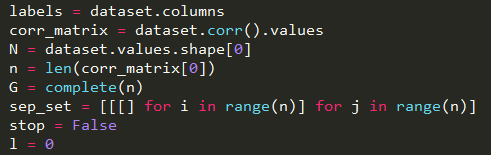
\includegraphics[scale=0.52]{img/initialization.PNG}
	\end{figure}

\end{frame}
\begin{frame}
\frametitle{Step 3: define adj() function}
\begin{itemize}
	\item Define the \textbf{adj()} function in order to get the adjacents of a node in a given graph.
\end{itemize}
	\begin{figure}[h!]
		\centering
		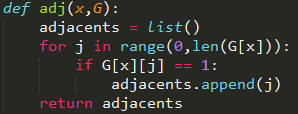
\includegraphics[scale=0.9]{img/adj.PNG}
	\end{figure}

\end{frame}
\begin{frame}
\frametitle{Step 4: how many variables are actually dependent?}
\begin{itemize}
	\item set stop condition to true
	\item retrieve dependent variables: i,j are actually dependent if the adjacence matrix[i][j] is equal to 1
	\item call the set of dependent variables \textbf{act\_dep}
\end{itemize}
	\begin{figure}[h!]
		\centering
		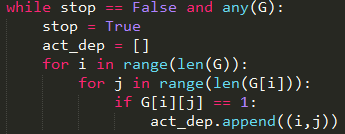
\includegraphics[scale=0.8]{img/depvar.PNG}
	\end{figure}

\end{frame}
\begin{frame}
\frametitle{Step 5: variables needed for independence test}
\begin{itemize}
	\item For \textbf{x,y} in \textbf{act\_dep};
	\item retrieve the \textbf{neighbors} of \textbf{x} calling the \textbf{adj()} function;
	\item remove y from the \textbf{neighbors} set;
	\item if \textbf{neighbors} set has dimension $\ge$ \textbf{l} then \begin{itemize}
	\item if \textbf{neighbors} set has dimension $>$ \textbf{l} go ahead.
	\end{itemize}
\end{itemize}
	\begin{figure}[h!]
		\centering
		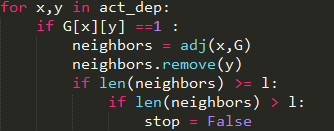
\includegraphics[scale=0.8]{img/indepvar.PNG}
	\end{figure}
\end{frame}
\begin{frame}
\frametitle{Step 6: conditional independence test}
\begin{itemize}
	\item Foreach set \textbf{K} of neighbors of dimension \textbf{l};
	\item test independence of \textbf{x} and \textbf{y} given \textbf{K};
	\item if the p value is greater than \textbf{alpha}:
	\begin{itemize}
		\item remove the edge x,y setting \textbf{G[x][y] = 0};
		\item set \textbf{K} as the \textbf{separation\_set[x][y]}.
	\end{itemize}
\end{itemize}
	\begin{figure}[h!]
		\centering
		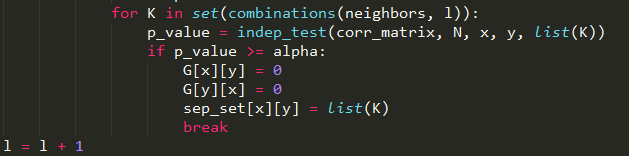
\includegraphics[scale=0.6]{img/indeptest.PNG}
		\label{Interfacce di un CS}
	\end{figure}
\end{frame}
\begin{frame}
\frametitle{Step 7: from the skeleton to the CPDAG}
\begin{itemize}
	\item Return \textbf{G} and \textbf{separation\_set};
	\item call \textbf{to\_cpdag(G, separation\_set)}.
\end{itemize}
	\begin{figure}[h!]
		\centering
		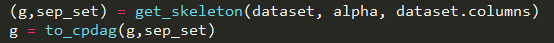
\includegraphics[scale=0.75]{img/tocpdag.PNG}
		\label{Interfacce di un CS}
	\end{figure}
\end{frame}

\begin{frame}
\frametitle{Step 8: define the getDependents() function}
\begin{itemize}
	\item Define \textbf{getDependents(adj\_matrix,reqij, reqji)};
	\item this function retrieve all the variables i,j such that: \textbf{adj\_matrix[i][j] == reqij} and \textbf{adj\_matrix[j][i] == reqji}.
\end{itemize}
	\begin{figure}[h!]
		\centering
		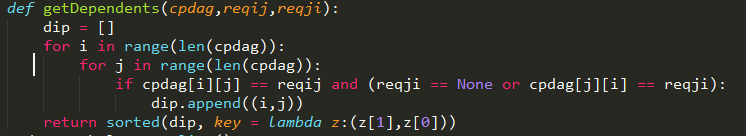
\includegraphics[scale=0.57]{img/getindep.PNG}
		\label{Interfacce di un CS}
	\end{figure}
\end{frame}

\begin{frame}
\frametitle{Step 9: CPDAG initialization}
\begin{itemize}
	\item Set the \textbf{cpdag} as the skeleton;
	\item set \textbf{dep} as the set of variables i,j for which exists an edge from i to j.
\end{itemize}
	\begin{figure}[h!]
		\centering
		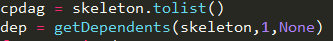
\includegraphics[scale=0.8]{img/cpdaginit.PNG}
		\label{Interfacce di un CS}
	\end{figure}
\end{frame}
\begin{frame}
\frametitle{Step 10: rule "zero" (1)}
\begin{itemize}
	\item For each pair x,y in \textbf{dip}:
	\item add to \textbf{allZ} all the variables \textbf{z} for which exists an egde from \textbf{z} to \textbf{y} and \textbf{z is not x};
	\item if:\\\textbf{there is no edge between x and z}\\ \textbf{there is a separation set between x and z}\\\textbf{there is a separation set between z and x}\\\textbf{y is not in separation set between x and z} or \textbf{in separation set between z and x}, then:
	\item remove the edge from y to x and from z to y.
\end{itemize}
\end{frame}
\begin{frame}
\frametitle{Step 10: rule "zero" (2)}
	\begin{figure}[h!]
		\centering
		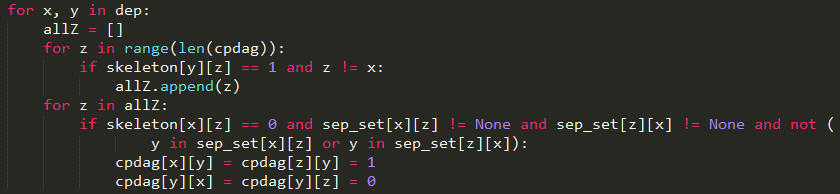
\includegraphics[scale=0.52]{img/rulezero.PNG}
		\label{Interfacce di un CS}
	\end{figure}
\end{frame}
\begin{frame}
\frametitle{Step 11: apply rules}
\begin{itemize}
	\item Using the same logic we apply the known rules 1,2 and 3;
	\begin{itemize}
		\item \textbf{Rule 1:} orient $j\;-\;k$ into $j \rightarrow k$ whenever there is an arrow  $i \rightarrow j$ such that $i$ and $k$ are not adjacent;
		\item \textbf{Rule 2:} orient $i\;-\;j$ into $i \rightarrow j$ whenever there is a chain $i \rightarrow k \rightarrow j$;
		\item \textbf{Rule 3:} orient $i\;-\;j$ into $i \rightarrow j$ whenever there are two chains $i \rightarrow k \rightarrow j$ and $i \rightarrow l \rightarrow j$ such that k and l are nonadjacent.
	\end{itemize}
	\item Return the resulting cpdag;
	\item using \textbf{matplotlib} and \textbf{networkx} we are able to plot the resulting cpdag.
\end{itemize}
%	\begin{figure}[h!]
%		\centering
%		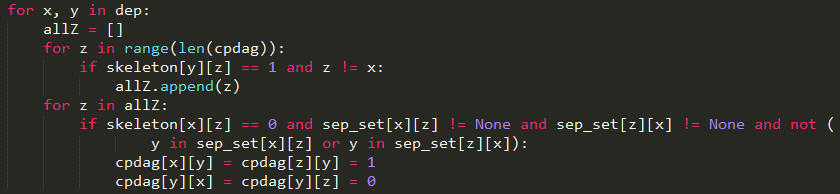
\includegraphics[scale=0.5]{img/rulezero.PNG}
%		\label{Interfacce di un CS}
%	\end{figure}
\end{frame}

\begin{frame}
\frametitle{Python vs R}
\begin{itemize}
	\item Consider this R code:
\end{itemize}
	\begin{figure}[h!]
		\centering
		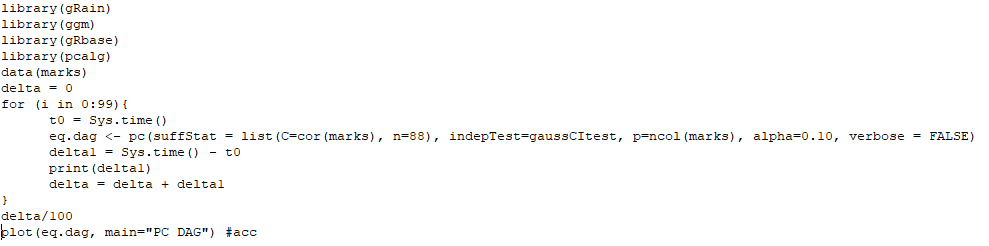
\includegraphics[scale=0.5]{img/r.PNG}
	\end{figure}
\begin{itemize}
	\item it gives:
	\end{itemize}
\end{frame}
\begin{frame}
\frametitle{Python vs R}
\begin{figure}[h!]
	\centering
	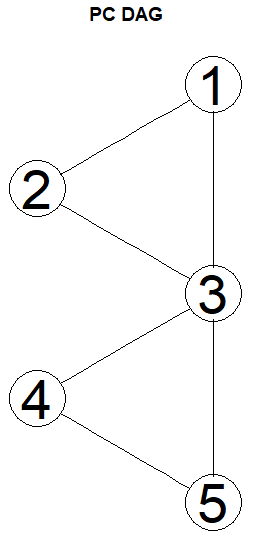
\includegraphics[scale=0.35]{img/rdag.PNG}
\end{figure}
\begin{figure}[h!]
	\centering
	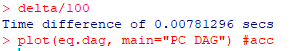
\includegraphics[scale=0.5]{img/rtime}
\end{figure}
\end{frame}
\begin{frame}
\frametitle{Python vs R}
\begin{itemize}
	\item Consider this python code:
	\end{itemize}
\begin{figure}[h!]
	\centering
	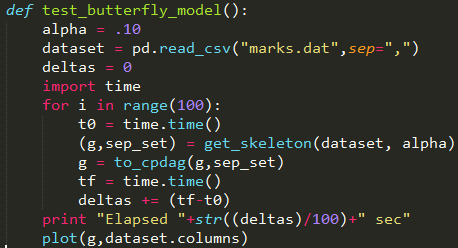
\includegraphics[scale=0.7]{img/py.PNG}
\end{figure}
\begin{itemize}
	\item it gives:
\end{itemize}
\end{frame}
\begin{frame}
\frametitle{Python vs R}
\begin{figure}[h!]
	\centering
	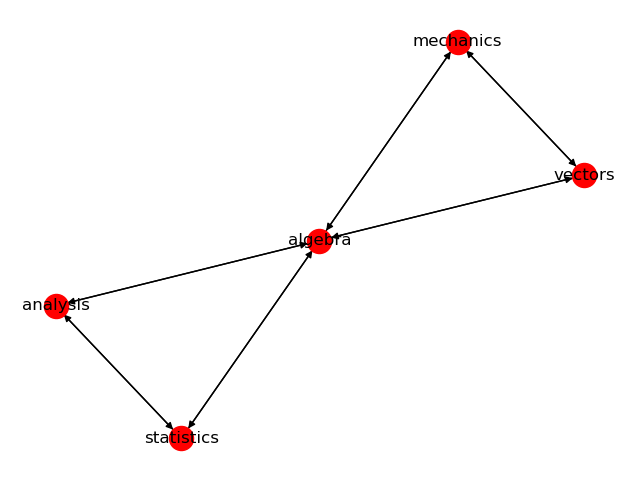
\includegraphics[scale=0.4]{img/pydag}
\end{figure}
\begin{figure}[h!]
	\centering
	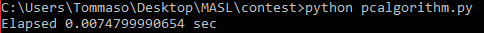
\includegraphics[scale=0.8]{img/pytime}
\end{figure}
\end{frame}

\begin{frame}
	\frametitle{Github repository}
	\begin{figure}[h!]
		\centering
		
\includegraphics[scale=0.15]{img/github.PNG}
	\end{figure}
	\begin{center}
		\color{blue}\href{https://github.com/alexfoglia1/MASL}{https://github.com/alexfoglia1/MASL}.
	\end{center} 
\end{frame}
\end{document}